\textit{Hybrid zero dynamics} is the term used to describe the dynamics of the phase variable of an underactuated walker which is subject to virtual constraints. The hybrid zero dynamics of a system are derived from the full state dynamics of continuous phase of the system, the impact map and the virtual constraint.

\subsection{Dynamics of a general underactuated walker}
The general equation of motion of a nonlinear time-invariant physical system may be written as:
\begin{equation}\label{eqn:dynamics}
	M\left(q(t)\right)\ddot{q}(t) + C\left(q(t),\dot{q}(t)\right)\dot{q}(t)
	 + G\left(q(t)\right) = B\left(q(t)\right)u(t)
\end{equation}
where $M\left(q(t)\right)$ is the matrix of inertial terms, $C\left(q(t),\dot{q}(t)\right)$ is the matrix of Coriolis and centrifugal terms, $G\left(q(t)\right)$ is the gradient of the potential field and $B\left(q(t)\right)$ is some matrix which specifies the effect of control inputs $u(t)$. \\

As in \cite{hurmuzlu1994rigid}, we assume that the collisions at each footstep are purely inelastic and the impact map has the following form:
\begin{eqnarray}
	q\left(t^+\right) &=& Rq\left(t^-\right) \\
	\dot{q}\left(t^+\right) &=& R\Delta\left(q\left(t^-\right)\right)\dot{q}\left(t^-\right)
\end{eqnarray} ~\\

For the underactuated walkers considered in this thesis, $R$ represents a relabelling of coordinates. An example is shown of such relabelling for the simple compass gait walker in Figure~\ref{fig:relabelimpact}.

\begin{figure}[htp]
	\centering
	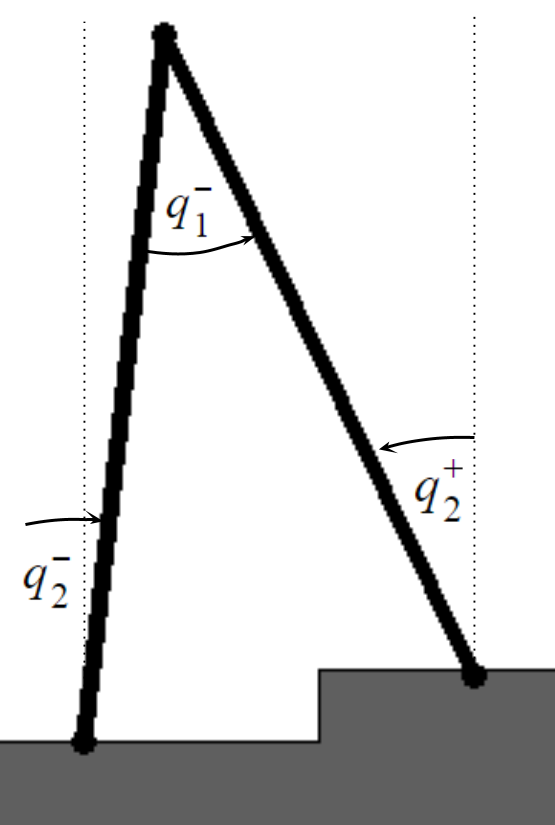
\includegraphics[scale=1]{3TechBackground/impact.png}
	\caption{Change of coordinates at impact}
	\label{fig:relabelimpact}
\end{figure}

\subsection{Application of virtual constraints and zero dynamics}
The application of virtual holonomic constraints is a method by which a system's generalised coordinates may be synchronised to a single coordinate, called the \textit{phase variable}, $\theta$. In order for this to be sensible, we assume that $\theta$ is increasing over some interval $[\theta_0, \theta_f]$. Under that assumption, we may construct functions for all of the generalised coordinates of the form:
\begin{equation}
	q_i(t) = \phi_i\left(\theta(t)\right), ~~ i = 1,2,\ldots,n
\end{equation}
Using trivial differentiation rules, we obtain
\begin{eqnarray}
	\dot{q}_i(t) &=& \frac{\partial\phi_i\left(\theta(t)\right)}{\partial\theta}\dot{\theta},
						~~i = 1,2,\ldots,n \\
	\ddot{q}_i(t) &=& \frac{\partial^2\phi_i\left(\theta(t)\right)}{\partial\theta^2}\dot{\theta}^2 +
						\frac{\partial\phi_i\left(\theta(t)\right)}{\partial\theta}\ddot{\theta},
						~~i = 1,2,\ldots,n
\end{eqnarray}
We define the following vector functions:
\begin{eqnarray}
	\Phi\left(\theta\right) &=& \left[ \phi_1\left(\theta\right), \phi_2\left(\theta\right), \ldots,
	\phi_n\left(\theta\right)\right]^T \\
	\Phi'\left(\theta\right) &=& \left[ \frac{\partial\phi_1\left(\theta\right)}{\partial\theta},
	\frac{\partial\phi_2\left(\theta\right)}{\partial\theta}, \ldots ,
	\frac{\partial\phi_n\left(\theta\right)}{\partial\theta} \right]^T \\
	\Phi''\left(\theta\right) &=& \left[ \frac{\partial^2\phi_1\left(\theta\right)}{\partial\theta^2},
	\frac{\partial^2\phi_2\left(\theta\right)}{\partial\theta^2}, \ldots ,
	\frac{\partial^2\phi_n\left(\theta\right)}{\partial\theta^2} \right]^T
\end{eqnarray} ~\\

Under the assumption perfect regulation of the virtual constraints, thus the above relations holding, we can evaluate the zero dynamics by simple substitution into Equation~\ref{eqn:dynamics}:
\begin{equation}
	M\left(\Phi(\theta)\right)\left[\Phi'(\theta)\ddot{\theta} + \Phi''\dot{\theta}^2\right] + 
	C\left(\Phi(\theta),\Phi'(\theta)\dot{\theta}\right)\Phi'(\theta)\dot{\theta} +
	G\left(\Phi(\theta)\right) = B\left(\Phi(\theta)\right)u_c
\end{equation}
where $u_c$ is the control which achieves perfect regulation of the constraints. This may be rearranged into a more convenient form:
\begin{equation} \label{eqn:zerodyn}
	\alpha(\theta)\ddot{\theta} + \beta(\theta)\dot{\theta}^2 + \gamma(\theta) = 0
\end{equation}
where, if we denote $B^{\perp}(q)$ as a row vector which satisfies $B^{\perp}(q)B(q)u_c = 0$,
\begin{eqnarray}
	\alpha(\theta) &=& B^{\bot}\left(\Phi(\theta)\right)M\left(\Phi(\theta)\right)\Phi'(\theta)\nonumber \\
	\beta(\theta) &=& B^{\bot}\left(\Phi(\theta)\right)\left(M\left(\Phi(\theta)\right)\Phi''(\theta)
		+C\left(\Phi(\theta),\Phi'(\theta)\right)\Phi'(\theta) \right) \nonumber \\
	\gamma(\theta) &=& B^{\bot}\left(\Phi(\theta)\right)G\left(\Phi(\theta)\right)
\end{eqnarray}

\subsection{Partial closed-form solutions for velocity and energy}
One of the useful properties of virtual constraints is the ability that they lend the designer of a motion planner to precompute a partial closed-form solution for velocity and energy. The solution is partial in that we obtain an expression for $\dot{\theta}^2$ in terms of $\theta$, rather than $\theta$ in terms of time. Under the assumption that $\theta$ is monotonic, it can be used as a new dependent variable:
\begin{eqnarray}
	\frac{d}{d\theta}\left[\dot{\theta}\left(t(\theta)\right)^2\right] &=& 
	\frac{d}{dt}\frac{dt}{d\theta}\left[\frac{d\theta}{dt}\left(t(\theta)\right)^2\right] \nonumber \\ 
	&=& 2\ddot{\theta}\left(t(\theta)\right)
\end{eqnarray}
Substituting Equation~\ref{eqn:zerodyn} into this expression, we arrive at a first-order ODE in $\dot{\theta}(\theta)^2$:
\begin{equation}\label{eqn:zerodynDE}
	\frac{d}{d\theta}\dot{\theta}(\theta)^2 = -2\frac{\beta(\theta)}{\alpha(\theta)}
		\dot{\theta}(\theta)^2 - 2\frac{\gamma(\theta)}{\alpha(\theta)}
\end{equation}
If we assume, as in \cite{manchester13planning}, that for all $\theta \in [\theta_0, \theta_f]$, we have local instantaneous controllability, i.e. $\alpha(\theta) \neq 0$, then we may solve Equation~\ref{eqn:zerodynDE} numerically over $[\theta_0, \theta_f]$, which yields an affine solution, i.e.
\begin{equation}
	\dot{\theta}(\theta)^2 = \Gamma(\theta, \theta_0)\dot{\theta}_0^2 + \Psi(\theta, \theta_0)
\end{equation}
From this, we may also derive the total mechanical energy of the system. For general systems with dynamics as expressed in Equation~\ref{eqn:dynamics}, the mechanical energy has the form:
\begin{equation}
	H\left(q,\dot{q}\right) = \dot{q}^TM(q)\dot{q} + V(q)
\end{equation}
Under perfectly regulated virtual constraints, this reduces to:
\begin{equation}
	\bar{H}\left(\theta,\dot{\theta}\right) := \Upsilon(\theta)\dot{\theta}^2 + \Xi(\theta)
\end{equation}
where
\begin{eqnarray*}
	\Upsilon(\theta) &=& \Phi'(\theta)^TM\left(\Phi(\theta)\right)\Phi'(\theta) \\
	\Xi(\theta) &=& V\left(\Phi(\theta)\right)
\end{eqnarray*}
Since this is affine in $\dot{\theta}^2$ for a given $\theta$, we may trivially calculate the closed form:
\begin{equation}
	H\left(\theta, \dot{\theta}\right) =
	\Upsilon(\theta)\Gamma\left(\theta,\theta_0\right)\dot{\theta}_0^2 +
	\Upsilon(\theta)\Psi\left(\theta,\theta_0\right) + \Xi(\theta)
\end{equation}

\subsection{B{\'e}zier curves as virtual constraints}
Bézier curves provide a way to produce families of curves for particular start and end heights and are sparsely identified by only $n+1$ points, where $n$ is the degree of the curve. These points provide an intuitive way of defining the curve, in contrast with polynomial coefficients.
\par

Theoretically, these curves need only be defined from the start to the endpoint of the continuous-phase which they specify. However, since the curve provides a virtual constraint to be enforced by a controller, it is necessary to define the curve over the full range of possible motion, here considered to be $\theta_1 \in \left[0, \pi\right]$, else it is possible for the walker to enter a region where the control signal is undefined. If we assume that the overshoot past the desired endpoint is small, then the shape of the curve should be flat outside the defined region. That is, when we leave the target region, we wish to set $\theta_2$ to the closest defined $\theta_2$. \\ \par

For the compass-gait walker, a general Bézier curve is defined by the following parametric equation.
\begin{equation}
	\begin{bmatrix}
		\theta_1 \\ \theta_2
	\end{bmatrix}
	=
	\sum_{i=0}^{n}\binom{n}{i}\left(1-t\right)^{n-i}t^i
	\begin{bmatrix}
		\theta_{1_i} \\ \theta_{2_i}
	\end{bmatrix} \label{eqn:genBez}
\end{equation}
Since this equation is not monotonic in $\theta_1$, it is not a convenient expression. Therefore, we build families of Bézier curves with the following formulation:
\begin{eqnarray}
	t &=& \frac{\theta_1 - \theta_{1_0}}{\theta_{1_n} - \theta_{1_0}} \\
	\theta_2 &=& \sum_{i=0}^{n}\binom{n}{i}\left(1-t\right)^{n-i}t^i\theta_{2_i}
\end{eqnarray}
This is expressible explicitly as
\begin{equation}
	\theta_2 = \frac{1}{\left(\theta_{1_n} - \theta_{1_0}\right)^n}\sum_{i=0}^{n}\binom{n}{i}
		\left(\theta_{1_n} - \theta_1\right)^{n-i}
		\left(\theta_1 - \theta_{1_0}\right)^i\theta_{2_i} \label{eqn:expBez}
\end{equation}
This formulation removes our ability to arbitrarily define the control points $\left(\theta_{1_i}, \theta_{2_i}\right)$, other than the endpoints. That is, this formulation produces curves of the form given in Equation~\ref{eqn:genBez} with
\begin{equation}
	\theta_{1_i} = \frac{i}{n}\left(\theta_{1_n}-\theta_{1_0}\right) + \theta_{1_0} ~~
	\forall ~~ i \in \left[1,~n-1\right]
\end{equation}

Since we can only define one of the two variables in each control point, to yield arbitrary curves of order $n$, before achievable with $n - 1$ free control points (i.e. non-endpoint control points), now requires $2n - 2$ such points. Since it is desirable to have the ability to set the gradient of approach to the control points independently of the shape of the polynomial (achievable using a general cubic Bézier curve) we use a quintic curve in the new formulation. This requires six control points.